% !TeX root = ../../thesis.tex
\chapter{Advanced model with kinetics}\label{ch:kinetics}


\begin{shaded}
This chapter is based on a manuscript prepared to be submitted:\\
M. Barzegari, C. Wang, S.V. Lamaka, G. Zavodszky, and L. Geris, ``Interface-coupled multiphysics computational modeling of local pH changes during the biodegradation of magnesium biomaterials.''
\end{shaded}

\section{Introduction}

Mg is the most studied biodegradable metal \cite{Liu2019,Zheng2014,Chen2014,Zhang2013}, on which many research groups have performed valuable biodegradation studies \cite{Esmaily2017,Li2016,Atrens2020,Kirkland2012}. The biodegradation behavior of Mg is investigated in \textit{in vitro} corrosion tests, in which the selection of the corrosive media plays an important role since it affects the underlying chemical reactions \cite{Mei2020}. By considering the main application of the biomaterial, which can be tissue engineering scaffolds, vascular stents, or orthopedic fixation implants, the corrosive media can be selected to be a representative of the service environment. The most basic form of the medium is a saline (NaCl) solution, in which the degradation rate is the highest possible \cite{Mei2020}. More complex solutions can be used to mimic the behavior of body environment by taking into account more body fluid components, the most popular of which are the Ringer's solution, PBS (phosphate buffered saline), SBFs (simulated body fluids), HBSS (Hank's balanced salt solution), and Earle's balanced salt solution (EBSS) \cite{Mei2020}. Adding more organic components to the solution will make it ready to simulate cell culture conditions. The common media for this purpose are MEM (Minimum Essential medium) and DMEM (Dulbecco's modified Eagle's medium) \cite{Mei2020}.

A wide range of various studies have already investigated the effect of different components in the aforementioned corrosive media on the degradation behavior of Mg materials \cite{Mei2019,Zeng2014,Johnston2017, Lamaka2018,Mei2019a}. A typical composition of "simulated body fluid" solutions (such as SBF, HBSS, and EBSS) is chloride, carbonate, phosphates, sulfate, and calcium. The individual effect of these components on the rate of degradation of Mg has been extensively studied, in which it has been observed that carbonate and phosphate slow down the rate while the effect of sulfate is negligible \cite{Johnston2017,Mei2019a}. The concentration of $\mathrm{HCO}_{3}^{-}$ affects the pH buffering capacity and the degradation rate of Mg simultaneously \cite{Xin2011}.

The effect of calcium ion is more complex because it has been found that $\mathrm{Ca}^{2+}$ doesn't contribute to the Mg corrosion directly \cite{Willumeit-Roemer2019}, but a mixed effect of $\mathrm{Ca}^{2+}$, $\mathrm{Mg}^{2+}$, $\mathrm{HCO}_{3}^{-}$, and $\mathrm{H}_{2} \mathrm{PO}_{4}^{-} / \mathrm{HPO}_{4}^{2-}$ forms a co-precipitation layer on the corroded surface of Mg, slowing down the corrosion rate of commercially pure Mg as well as some the of the Mg alloys \cite{Mei2019,Lamaka2018}. It has been also reported that although various Mg alloys show different intrinsic degradation behavior in NaCl solution, they possibly behave similarly in simulated body fluids \cite{Agha2016,Mei2019a}. Since the humoral regulations inside the human body control the changes in pH of body fluids, it's common to use pH buffers to mimic a similar condition, but it should be taken into account that buffering solution may affect the degradation rate of Mg \cite{Cui2017,Kannan2017}. pH buffers may also delay the formation of the precipitate layer \cite{Lamaka2018}. An alternative solution to address this issue is to use natural pH buffers such as $\mathrm{HCO}_{3}^{-}/\mathrm{CO}_{2}$, a technique that is commonly used for immersion tests under cell culture conditions. In this situation, an equilibrium between $\mathrm{H}_{2} \mathrm{CO}_{3}\left(\mathrm{CO}_{2}\right)$, $\mathrm{HCO}_{3}{ }^{-}$, and $\mathrm{CO}_{3}{ }^{2-}$ keeps the pH constant. As a result, using simulated body fluids for corrosion tests without additional synthetic pH buffer is still acceptable \cite{Lamaka2018,Mei2019a}.

The major reactions occurring in simulated body fluids can be written as:
\begin{equation}
\mathrm{Mg}+2 \mathrm{H}_{2} \mathrm{O} \rightarrow \mathrm{Mg}(\mathrm{OH})_{2}+\mathrm{H}_{2}
\end{equation}
\begin{equation}
2 \mathrm{Mg}+2 \mathrm{H}_{2} \mathrm{O}+\mathrm{O}_{2} \rightarrow 2 \mathrm{Mg}(\mathrm{OH})_{2}
\end{equation}
\begin{equation}
5 \mathrm{Ca}^{2+}+3 \mathrm{PO}_{4}^{3-}+\mathrm{OH}^{-} \rightarrow \mathrm{Ca}_{5}\left(\mathrm{PO}_{4}\right)_{3} \mathrm{OH}
\end{equation}
\begin{equation}
\mathrm{Ca}^{2+}+2 \mathrm{OH}^{-} \rightarrow \mathrm{Ca}(\mathrm{OH})_{2}
\end{equation}
\begin{equation}
\mathrm{Mg}^{2+}+\mathrm{CO}_{3}^{2-} \rightarrow \mathrm{MgCO}_{3}
\end{equation}
\begin{equation}
\mathrm{Ca}^{2+}+\mathrm{CO}_{3}^{2-} \rightarrow \mathrm{CaCO}_{3}
\end{equation}
\begin{equation}
 3 \mathrm{Mg}^{2+}+2 \mathrm{PO}_{4}^{3-} \rightarrow \mathrm{Mg}_{3}\left(\mathrm{PO}_{4}\right)_{2}
\end{equation}
\begin{equation}
\mathrm{CO}_{3}^{2-}(a q)+H^{+}(a q) \rightarrow \mathrm{HCO}_{3}^{-}(a q)
\end{equation}
\begin{equation}
P O_{4}^{3-}(a q)+H^{+}(a q)\rightarrow \mathrm{HPO}_{4}^{2-}(a q)
\end{equation}

Then, the aforementioned protection layer is formed on the corroded surface as a hydroxyapatite-like precipitation according the following reaction \cite{Atrens2015,Song2009,Silva2018,Jiang2019}:
\begin{equation} \label{eq:kinetics_hydrox_react}
\begin{aligned}
m \mathrm{Mg}^{2+}+n \mathrm{Ca}^{2+}&+x \mathrm{H}_{2} \mathrm{PO}_{4}^{-} / \mathrm{HPO}_{4}^{2-}+y \mathrm{HCO}_{3}^{-}+z \mathrm{OH}^{-}\\
& \rightarrow \mathrm{Mg}_{m} \mathrm{Ca}_{n}\left(\mathrm{PO}_{4}\right)_{x}\left(\mathrm{CO}_{3}\right)_{y}\left(\mathrm{OH}^{-}\right)_{z}
\end{aligned}
\end{equation}

In fact, the similarity in corrosion behavior of various Mg alloys in SBF solutions is because of the similar composition of this quasi-protective layer, a mechanism that doesn't occur in NaCl solution, leading to more apparent difference of degradation rate between Mg alloys. The composition of the formed hydroxyapatite-like precipitation layer is close to the ones found \textit{in vivo} \cite{Mei2020}. Additionally, local pH measurements in HBSS and SBF shows that in contrast to saline solutions, the local pH value is not alkaline \cite{Lamaka2018,Mei2021}. This has been reported for hydrodynamics situation, under which the medium composition is kept constant by replacing the consumed ions by means of fluid flow.

Building mathematical and computational models of the biodegradation process in complex buffered solutions can help saving resources required to perform \textit{in vitro} tests, but the details of the aforementioned chemistry is difficult to capture in a mechanistic model. Few attempts have been made to model the underlying chemical reactions in SBF solutions \cite{Hoche2014,Dolgikh2019,Zeller-Plumhoff2022}, but due to the complexity of the resulting mathematical models, it's not feasible to extend them to 3D and real-world cases, like for simulation of the degradation of biomedical implants. In case of data-driven approaches \cite{Zeller-Plumhoff2021}, the applicability is limited to the studied conditions, making it difficult for developed models to achieve high extensibility and generalizability. In the current study, a detailed mathematical model is presented to extend our previous work \cite{Barzegari2021}, in which a mechanistic model of the biodegradation process is coupled with a thermodynamics-based code to predict local interfacial biodegradation of Mg in HBSS solutions. The local pH changes is selected as the validation criterion to compare with experimental results. Besides other parameters affecting the Mg biodegradation mechanism, monitoring the pH changes at the degradation interface has proved to be important due to its direct effect on the formation and stability of the degradation products layer \cite{Gonzalez2021}.


\section{Results}

\subsection{Thermodynamics-based simulation}

Inputting the experimental conditions in the Hydra-Medusa software, including the initial composition and the contributing chemical components, results in a huge and complex output containing all the possible occurring chemical reactions. Out of this output, relevant reactions for the current biodegradation systems were filtered out, and the filtered reactions were converted to desired concentration units. Fig. \ref{fig:kinetics_medusa_profiles} depicts the output of this process separately for simulations performed at $25^{\circ}C$ (RT) and $37^{\circ}C$, showing how the concentration of relevant components vary with changing the environment pH. The solubility products of these simulations were taken from Table \ref{tab:kinetics_reactions}, and equilibrium concentrations were set to be equal to the composition of the electrolyte, listed in Table  \ref{tab:kinetics_electrolyte_composition}.

\begin{figure}[h]
\centering
\medskip
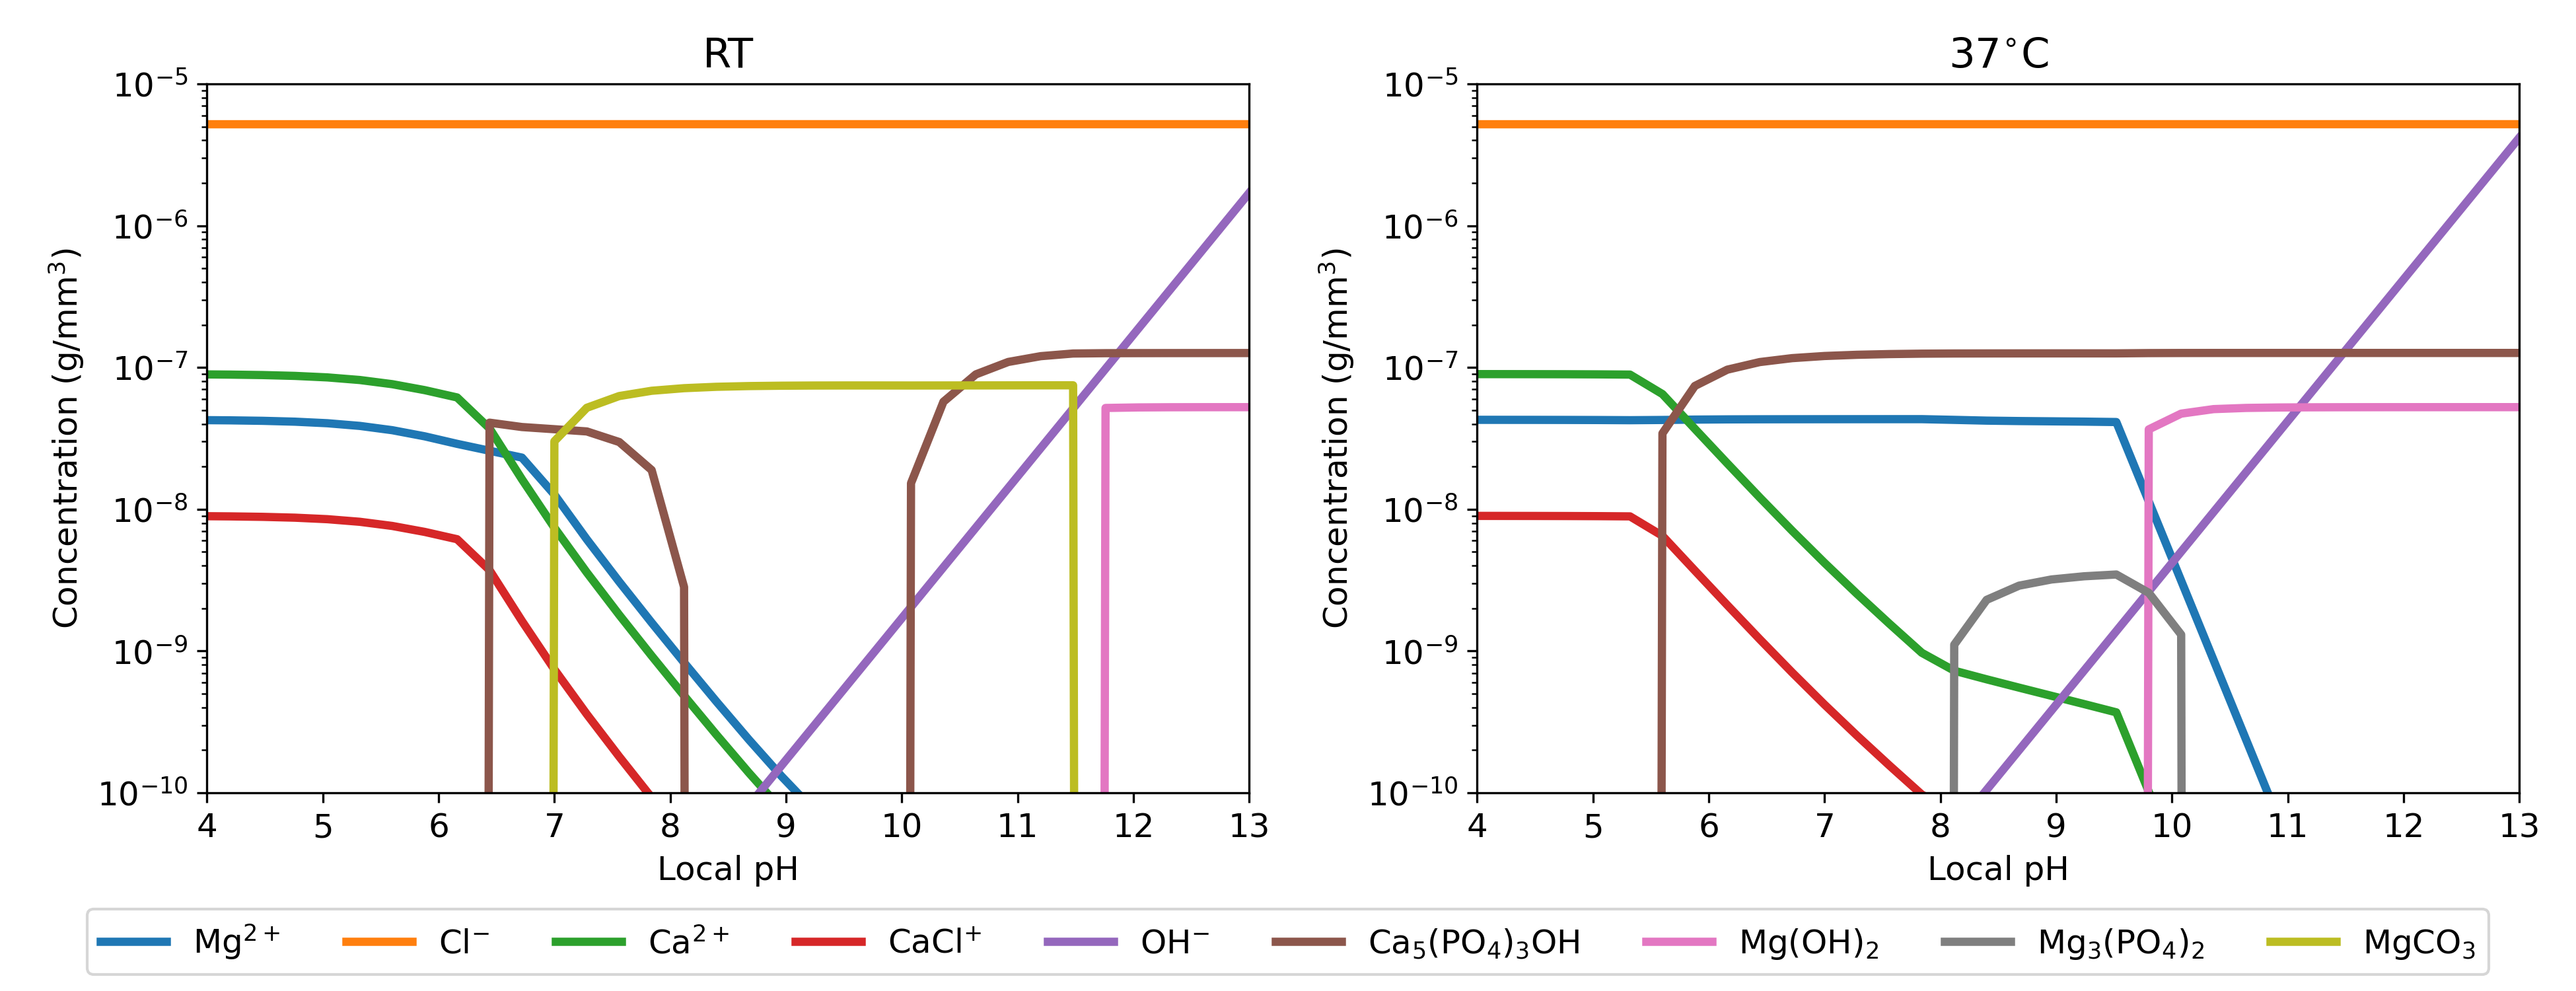
\includegraphics[width=\textwidth]{medusa_profiles.png}
\caption[Hydra-Medusa software output for given experimental conditions]{Selected relevant components from the Hydra-Medusa software output for given experimental conditions, showing how the concentration of various components vary with changing local pH} \label{fig:kinetics_medusa_profiles}
\end{figure}

\subsection{Biodegradation simulations}

Fig. \ref{fig:kinetics_local_ph_visual} shows a visualization of the local pH profiles from the top and side views for simulations performed at  $25^{\circ}C$ (RT) and $37^{\circ}C$ after 12 hours. These profiles are comparable with the local pH distribution measured in the experiments as shown in Fig. \ref{fig:kinetics_local_ph_experimental}. In these figures, the flow is from left to right, advecting the released ions in the flow direction.

\begin{figure}[h]
\centering
\medskip
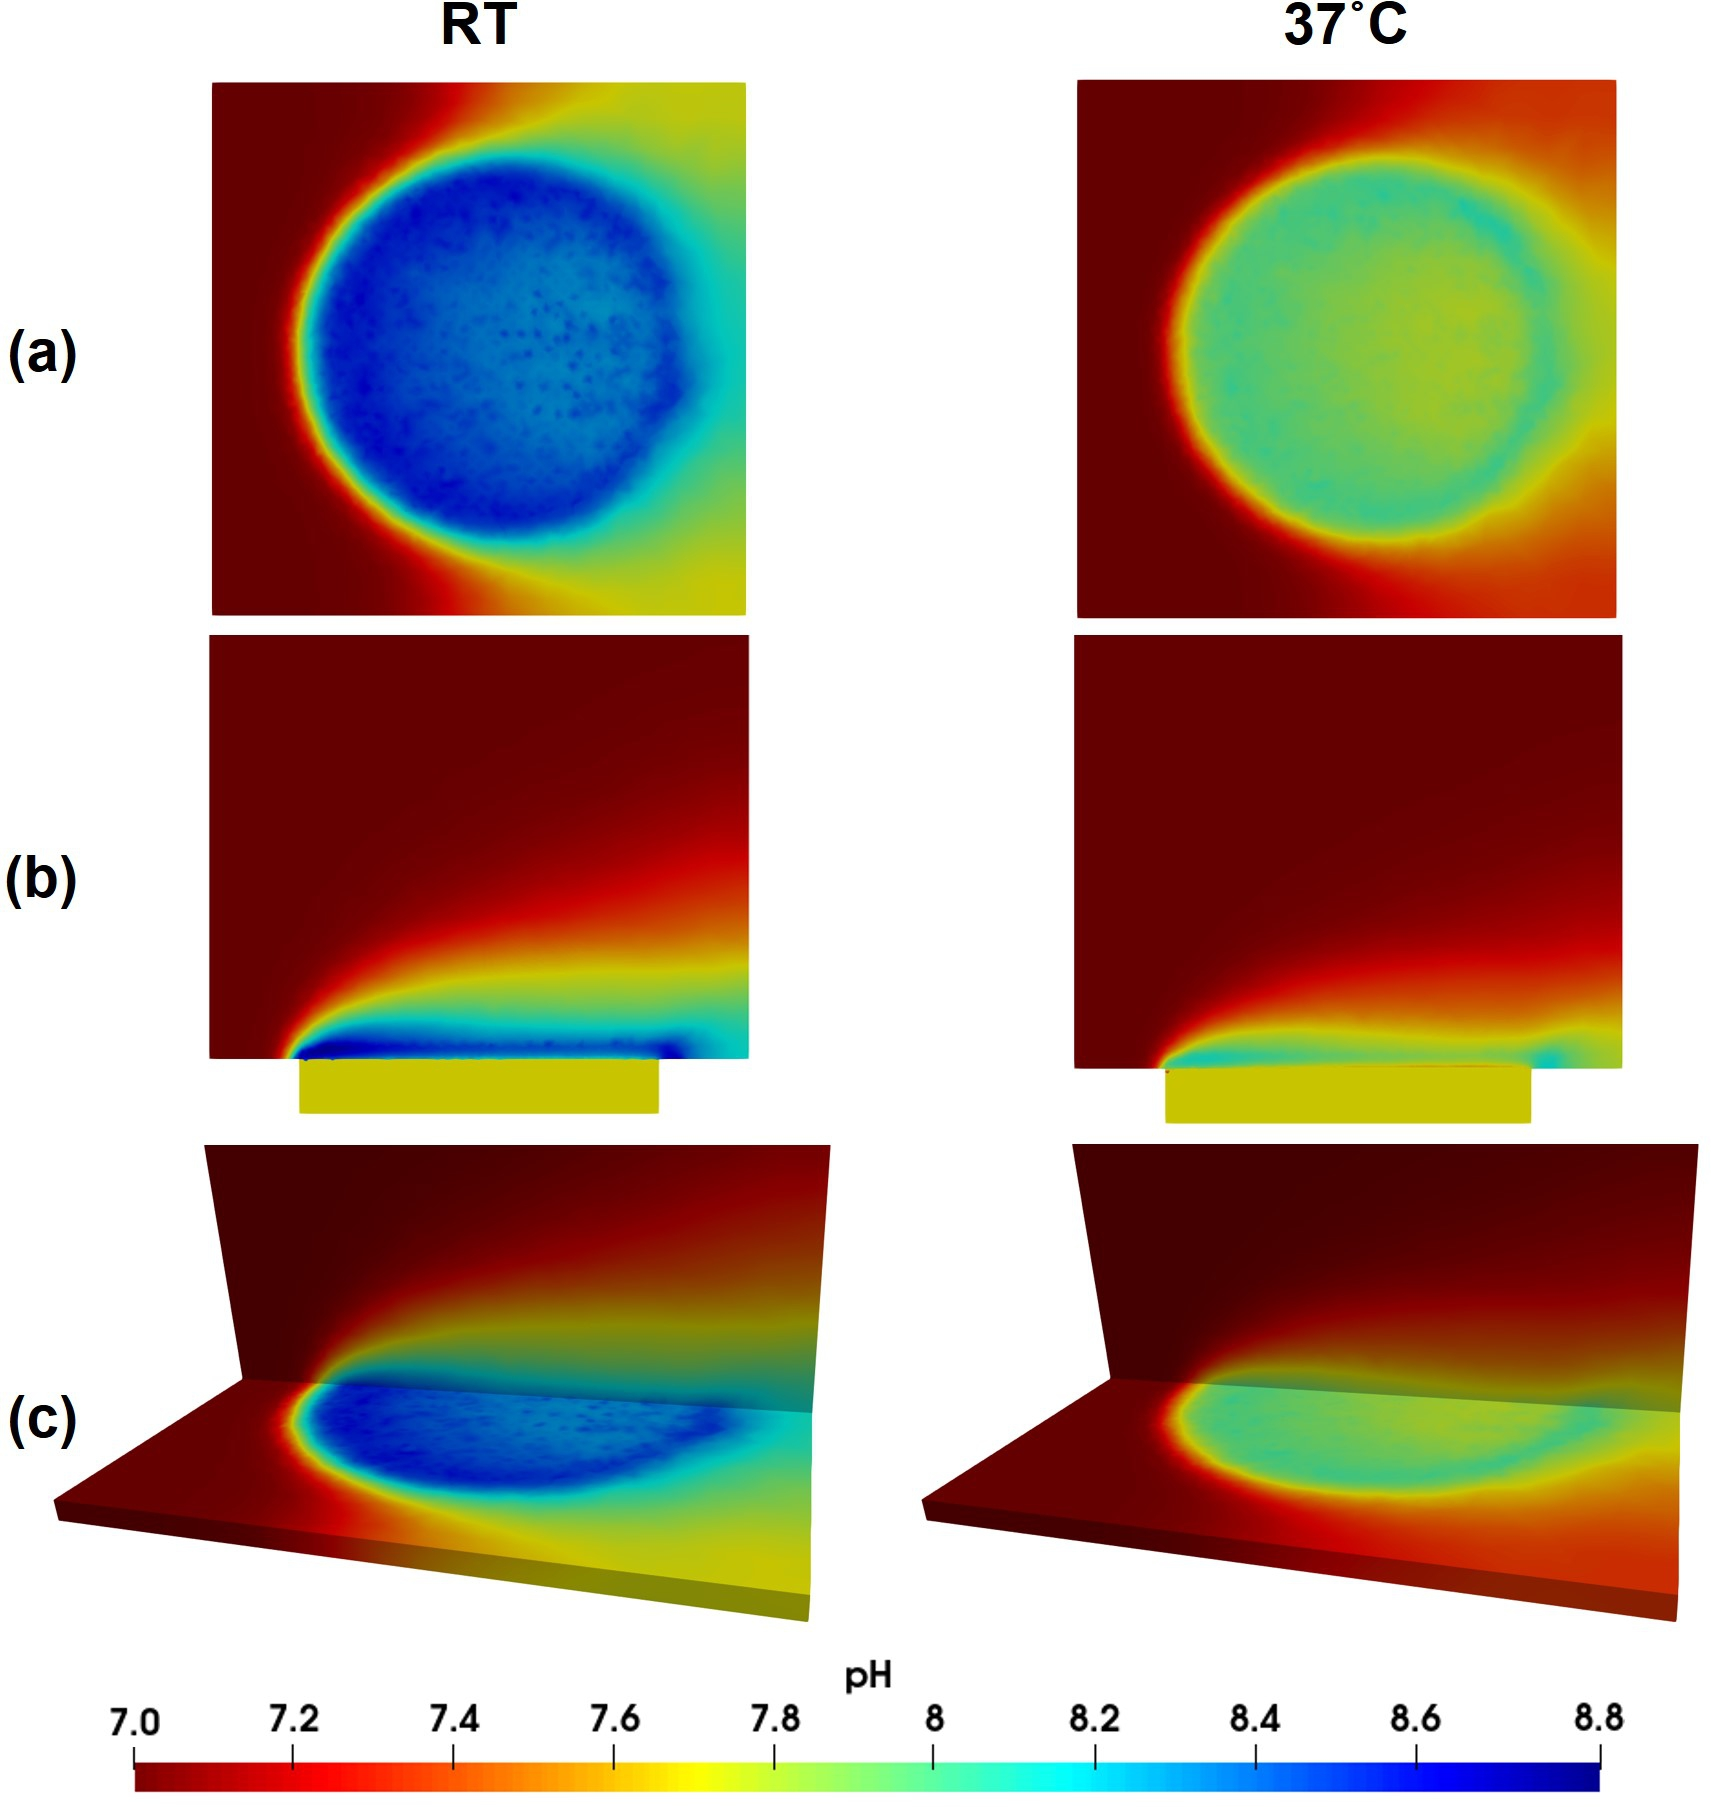
\includegraphics[width=\textwidth]{local_ph_visual.jpg}
\caption[Simulation results for local pH predictions]{Simulation results for local pH predictions, depicting the local pH in a) top view from a horizontal cross section, b) side view from a vertical cross section, and c) perspective view with both the top and side cross sections, for simulations performed at $25^{\circ}C$ (RT) and $37^{\circ}C$.} \label{fig:kinetics_local_ph_visual}
\end{figure}

\begin{figure}[h]
\centering
\medskip
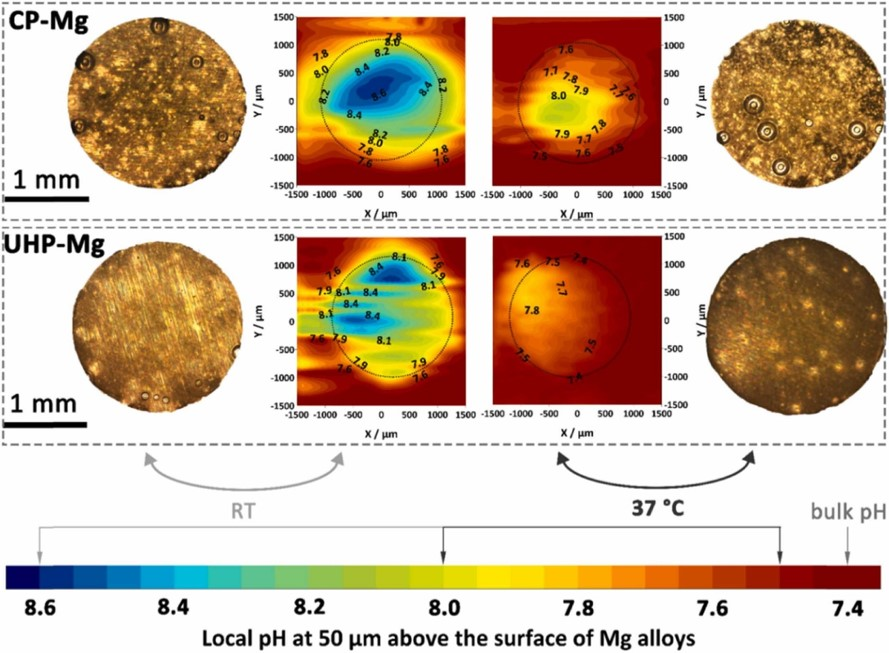
\includegraphics[width=\textwidth]{local_ph_experimental.jpg}
\caption[Experimental results for distribution of local pH above the sample]{Experimental results for distribution of local pH above the surface of the sample, measured after 12 hours of degradation.} \label{fig:kinetics_local_ph_experimental}
\end{figure}

Quantitative profiles provide a more accurate comparison between the computational predictions and experimentally-obtained values. The horizontal profiles, also called linescans, are depicted in Fig. \ref{kinetics_vertical_profile}, in which the local pH changes are plotted across a horizontal line $50 \mu\mathrm{m}$ above the surface of the sample for experiments using CP and UHP Mg and the computational model. The data is recorded after 12 hours of immersion, which was also the final time of the simulations.

\begin{figure}[h]
\centering
\medskip
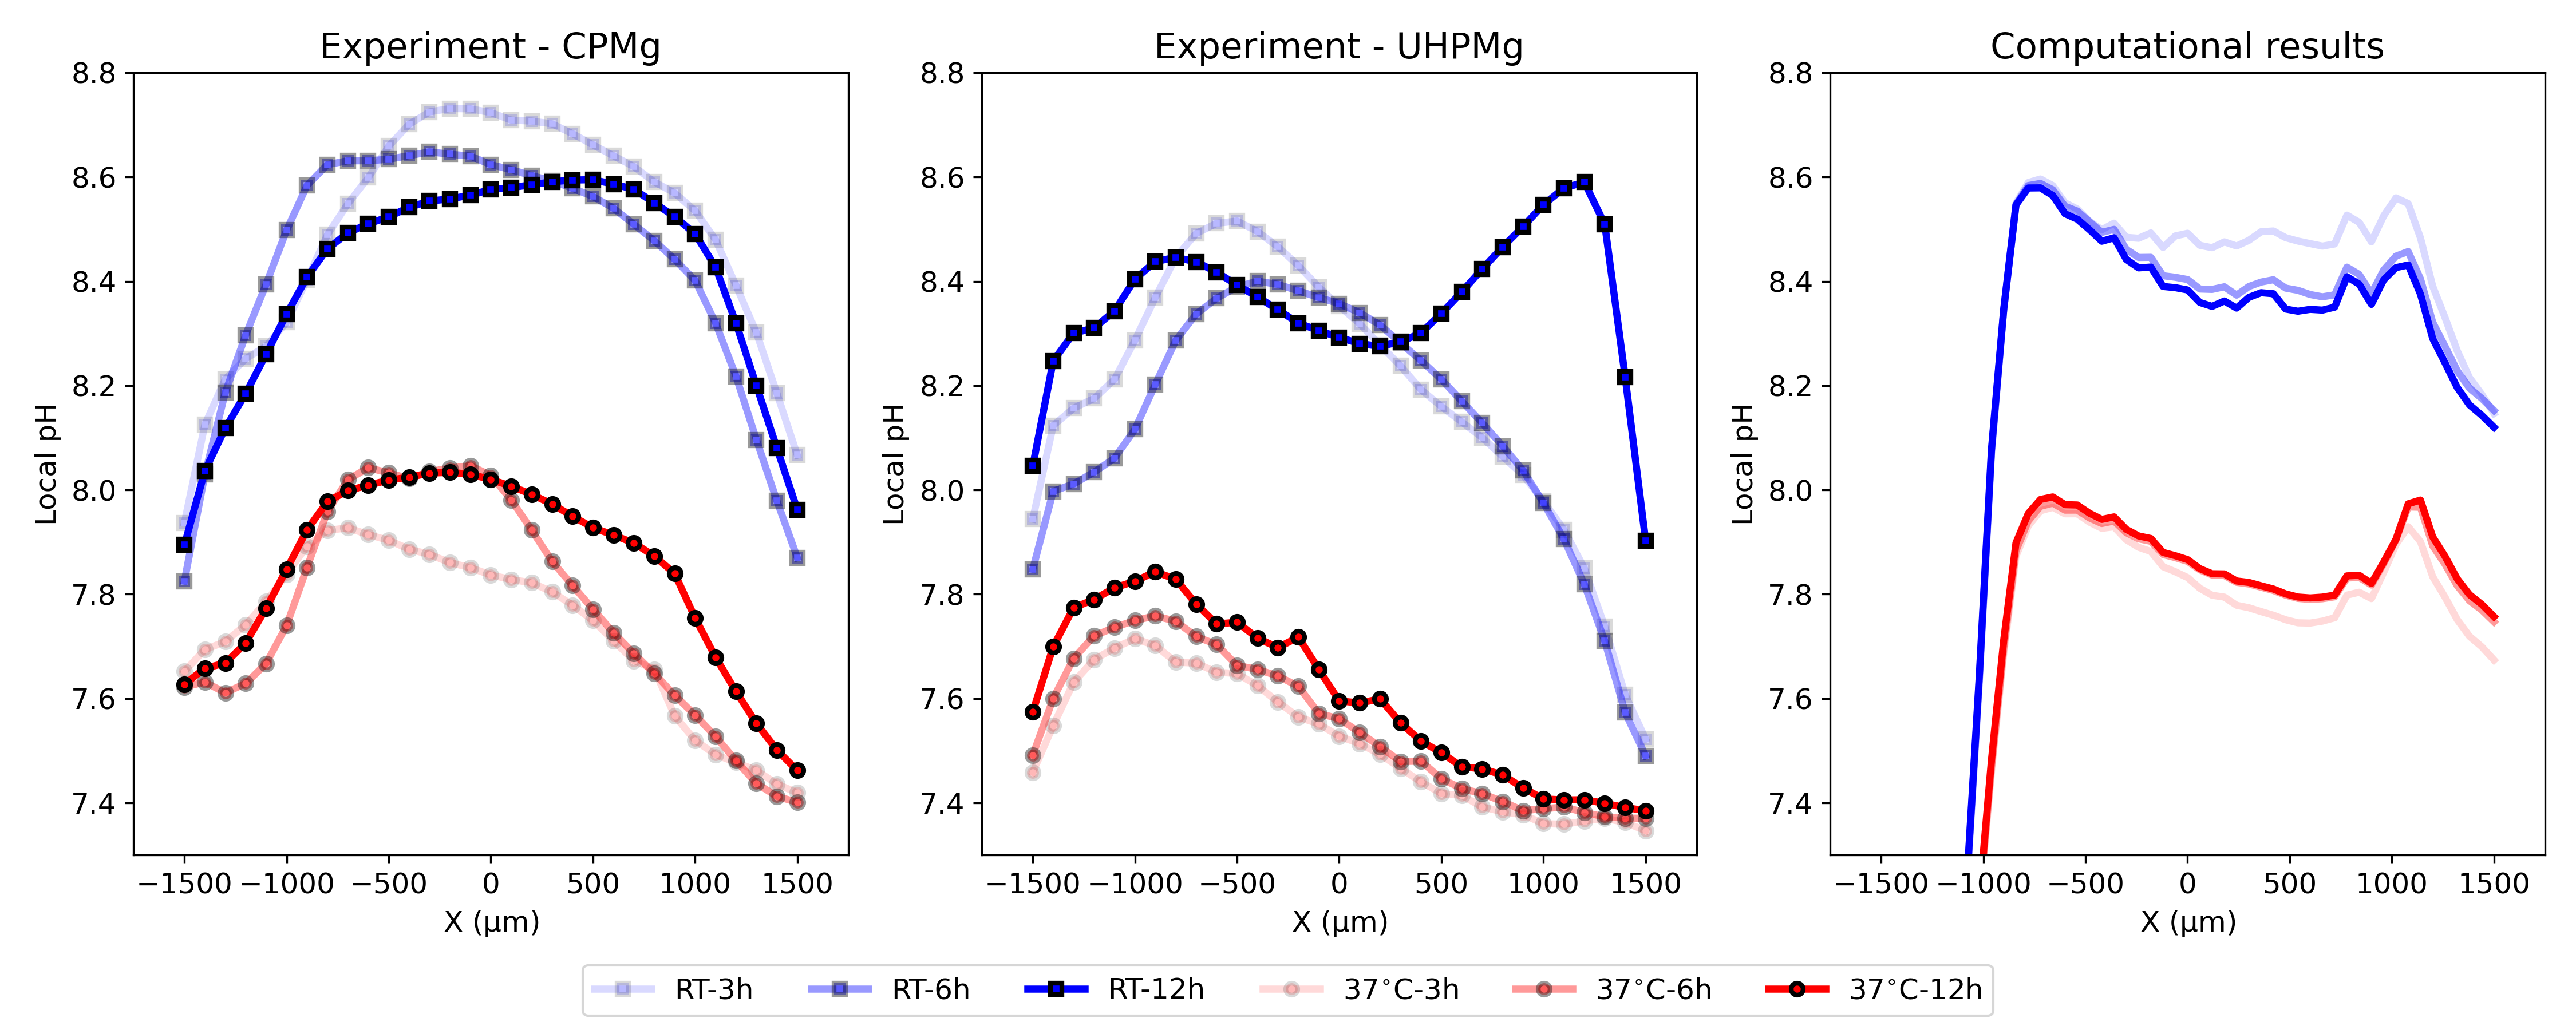
\includegraphics[width=\textwidth]{line_scans.png}
\caption[Comparing computational and experimental for horizontal line scans of local pH]{Comparing computational predictions and experimentally-obtained  horizontal line scans of local pH changes, measured $50 \mu\mathrm{m}$ above the surface of the sample after 12 hours of degradation.} \label{fig:kinetics_line_scans}
\end{figure}

Similarly, Fig. \ref{fig:kinetics_vertical_profile} demonstrates the vertical pH profile after 12 hours of degradation, where the local pH is measured over a distance of $0.5 \mathrm{mm}$ vertically, starting from $50 \mu\mathrm{m}$ above the sample.

\begin{figure}[h]
\centering
\medskip
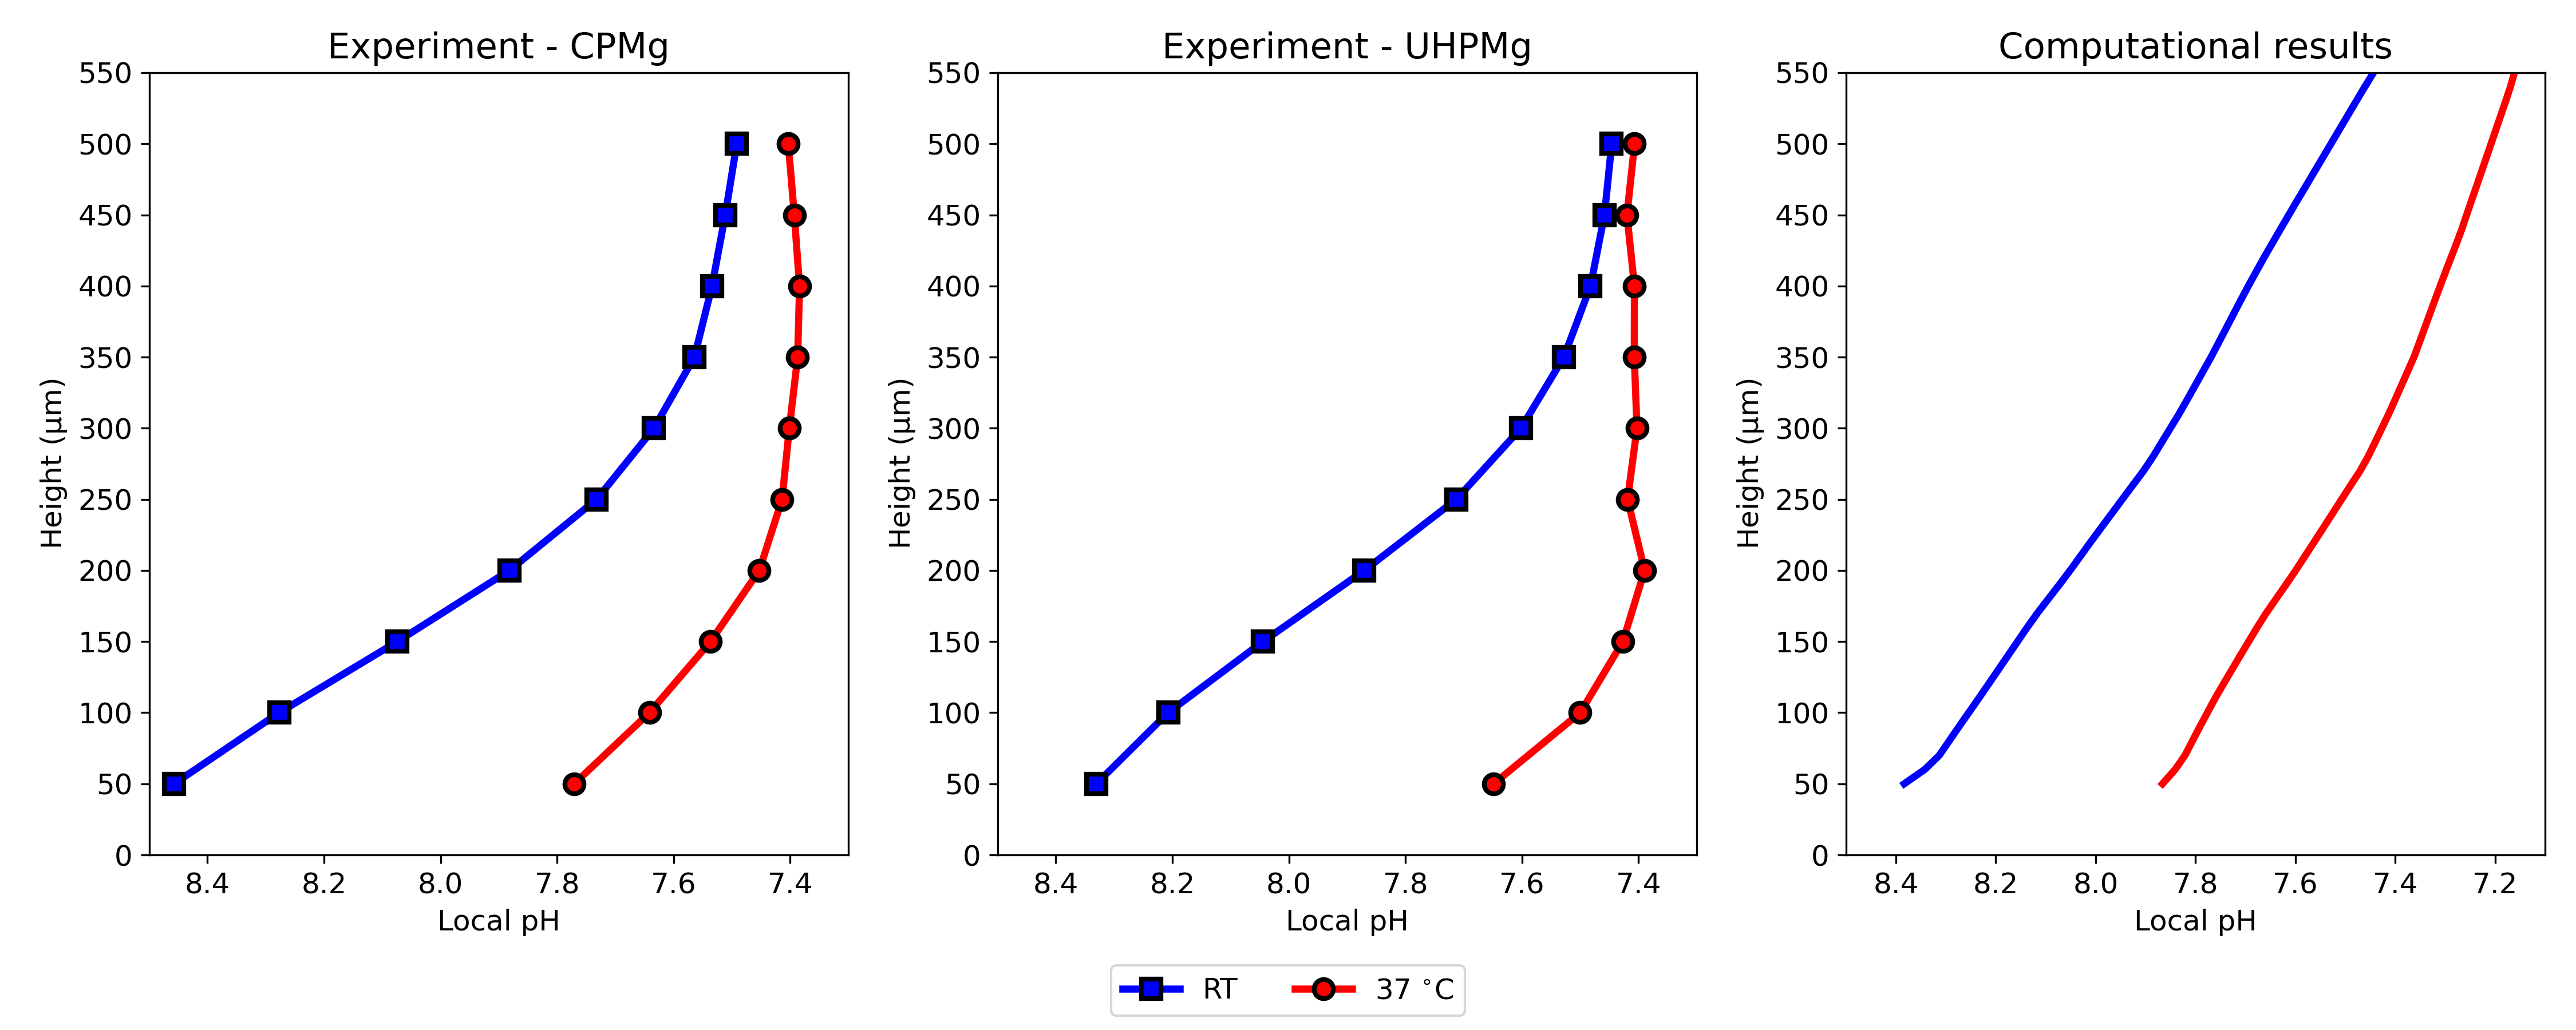
\includegraphics[width=\textwidth]{vertical_profile.png}
\caption[Comparing computational and experimental vertical pH profiles]{Comparing computational and experimental results for the local pH profiles, measured over a vertical line above the center of the sample after 12 hours of immersion.} \label{fig:kinetics_vertical_profile}
\end{figure}

\section{Discussion}

Dummy text for discussion.

\section{Methods}

\subsection{Experimental setup}

Dummy text for experimental setup.

\begin{table}[h]
\caption[Chemical composition of the HBSS electrolyte]{Chemical composition of the HBSS electrolytes used to perform corrosion tests for local pH measurements.}
\medskip
\centering
\begin{tabular}{cc}
\hline
{Components} & {mM} \\
\hline
$\mathrm{KCl}$ & 5.33 \\
$\mathrm{KH}_{2} \mathrm{PO}_{4}$ & 0.44 \\
$\mathrm{NaHCO}_{3}$ & 4.17 \\
$\mathrm{NaCl}$ & 137.9 \\
$\mathrm{Na}_{2} \mathrm{HPO}_{4}$ & 0.34 \\
$\mathrm{CaCl}_{2}$ & 1.26 \\
$\mathrm{MgCl}_{2} \cdot 6 \mathrm{H}_{2} \mathrm{O}$ & 0.49 \\
$\mathrm{MgSO}_{4} \cdot 7 \mathrm{H}_{2} \mathrm{O}$ & 0.41 \\
$\mathrm{D}-\mathrm{Glucose}$ & 5.56 \\
\hline

\end{tabular}
\label{tab:kinetics_electrolyte_composition}
\end{table}


\begin{table}[t]
\caption[The elemental composition of highly-pure and commercial-pure Mg]{The elemental composition of ultra high pure and commercial pure Mg used for performing corrosion experiments}
\medskip
\centering
\begin{tabular}{lcccccc}
\hline & {Fe} & {Si} & {Mn} & {Al} & {Cu} & {Ni} \\
\hline { CP-Mg } & 0.03420 & 0.0001 & 0.00237 & 0.00402 & 0.00037 & <0.0002  \\
{ UHP-Mg } & 0.0012 & <0.0001 & 0.00037 & 0.00291 & <0.0001 & <0.0002
\end{tabular}
\label{tab:kinetics_alloys_composition}
\end{table}


\begin{figure}[h]
\centering
\medskip
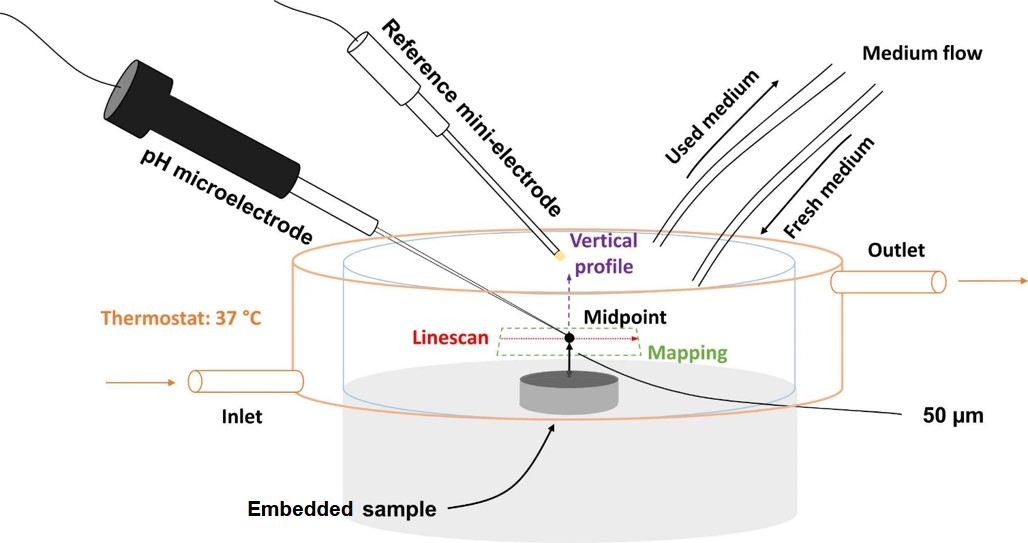
\includegraphics[width=0.9\textwidth]{setup.jpg}
\caption[Experimental setup for validating the coupled biodegradation model]{Experimental setup for validating the coupled biodegradation model} \label{fig:kinetics_setup}
\end{figure}

\subsection{Computational model construction}

The computational model in the current study comprises of 3 coupled components:
\begin{enumerate}
\item
An extended version of the mechanistic biodegradation model based on our previous work \cite{Barzegari2021} to obtain Mg and hydroxide ions distributions and initial formation of the protective layer based on the simplification assumptions.
\item
A thermodynamics-based simulation to estimate the concentration of various components of the electrolyte in regions close to the surface of the sample based on the calculated pH of component 1.
\item
A module to link the above 2 components and calculate the hydroxyapatite-like precipitation concentration, in which pH data were transfer from component 1 to component 2 for each node of the computational mesh to calculate the concentration of ions depending on the computed local pH and transfer back the calculated precipitation concentration to component 1.
\end{enumerate}

The computational model of the biodegradation was developed by deriving a set of reaction-diffusion-advection equations from the chemistry of the corrosion of Mg in hydrodynamics conditions. The following basic reactions are captured by this model, extended by splitting into more equations in comparison to our previous contribution \cite{Barzegari2021}:\begin{equation} \label{eq:kinetics_oxidation_react1}
\mathrm{Mg}+2 \mathrm{H}_{2} \mathrm{O} \stackrel{k_{0}}{\rightarrow} \mathrm{Mg}^{2+}+\mathrm{H}_{2}+2 \mathrm{OH}^{-}
\end{equation}
\begin{equation} \label{eq:kinetics_oxidation_react2}
\mathrm{Mg}^{2+}+2 \mathrm{OH}^{-} \stackrel{k_{1}}{\rightarrow} \mathrm{Mg}(\mathrm{OH})_{2}+\mathrm{H}_{2}
\end{equation}
\begin{equation} \label{eq:kinetics_break_react}
\mathrm{Mg}(\mathrm{OH})_{2}+2 \mathrm{Cl}^{-} \stackrel{k_{2}}{\rightarrow} \mathrm{Mg}^{2+}+2 \mathrm{Cl}^{-}+2 \mathrm{OH}^{-}
\end{equation}
\begin{equation} \label{eq:kinetics_break_react_mgo}
\mathrm{MgO}+ \mathrm{Cl}^{-} + \mathrm{H}_{2} \mathrm{O} \stackrel{k_{2}}{\rightarrow} \mathrm{Mg}^{2+}+ \mathrm{Cl}^{-}+ 2\mathrm{OH}^{-}
\end{equation}

The following state variables hold the concentration of various basic ions involved in reactions described by Eqs. \ref{eq:kinetics_oxidation_react1}, \ref{eq:kinetics_oxidation_react2}, \ref{eq:kinetics_break_react}, and \ref{eq:kinetics_break_react_mgo}:
\begin{equation} \label{eq:kinetics_state_vars_film}
\begin{aligned}
&C_{\mathrm{Mg}} = C_{\mathrm{Mg}}(\mathbf{x},t), \quad C_{\mathrm{Mg}_\mathrm{[s]}} = C_{\mathrm{Mg}_\mathrm{[s]}}(\mathbf{x},t), \quad C_{\mathrm{Mg}(\mathrm{OH})_{2}} = C_{\mathrm{Mg}(\mathrm{OH})_{2}}(\mathbf{x},t)  \\
&C_{\mathrm{Cl}} = C_{\mathrm{Cl}}(\mathbf{x},t), \quad C_{\mathrm{OH}} = C_{\mathrm{OH}}(\mathbf{x},t) \quad \mathbf{x} \in \Omega \subset \mathbb{R}^{3}
\end{aligned},
\end{equation}

Additionally, 2 more state variable are needed to couple the models, in which the calculated concentration of the hydroxyapatite-like precipitation as well as the cumulative layer concentration are held:
\begin{equation} \label{eq:kinetics_state_vars}
C_{\mathrm{Hydrox}} = C_{\mathrm{Hydrox}}(\mathbf{x},t), \quad C_{\mathrm{Film}} = C_{\mathrm{Film}}(\mathbf{x},t) \quad \mathbf{x} \in \Omega \subset \mathbb{R}^{3},
\end{equation}
where the total film concentration can be calculated as:
\begin{equation} \label{eq:kinetics_film_cumulative}
C_{\mathrm{Film}} = C_{\mathrm{Hydrox}} + C_{\mathrm{\mathrm{Mg}(\mathrm{OH})_{2}}}.
\end{equation}

With the above state variables defined, the basic biodegradation model can be constructed by deriving the following PDEs:
\begin{equation} \label{eq:kinetics_pde_mg_solid}
\frac{\partial C_{\mathrm{Mg}_\mathrm{[s]}}}{\partial t}=-k_{0}C_{\mathrm{Mg}_\mathrm{[s]}}
\end{equation}
\begin{equation} \label{eq:kinetics_pde_mg}
\frac{\partial C_{\mathrm{Mg}}}{\partial t}=\nabla \cdot \left(D_{\mathrm{Mg}}^{e}  \nabla C_{\mathrm{Mg}} \right)-\nabla \cdot \left({\mathbf u} C_{\mathrm{Mg}} \right)+k_{0}C_{\mathrm{Mg}_\mathrm{[s]}}-k_{1}\alpha C_{\mathrm{Mg}}C_{\mathrm{OH}}^2 +k_{2} C_{\mathrm{Film}} {C_{\mathrm{Cl}}}^{2}
\end{equation}
\begin{equation} \label{eq:kinetics_pde_film}
\frac{\partial C_{\mathrm{Mg}(\mathrm{OH})_{2}}}{\partial t}=k_{1}\alpha C_{\mathrm{Mg}}C_{\mathrm{OH}}^2 -k_{2} C_{\mathrm{Film}} {C_{\mathrm{Cl}}}^{2}
\end{equation}
\begin{equation} \label{eq:kinetics_pde_cl}
\frac{\partial C_{\mathrm{Cl}}}{\partial t}=\nabla \cdot \left(D_{\mathrm{Cl}}^{e}  \nabla C_{\mathrm{Cl}} \right)-\nabla \cdot \left({\mathbf u} C_{\mathrm{Cl}} \right)
\end{equation}
\begin{equation} \label{eq:kinetics_pde_oh}
\frac{\partial C_{\mathrm{OH}}}{\partial t}=\nabla \cdot \left(D_{\mathrm{OH}}^{e}  \nabla C_{\mathrm{OH}} \right)-\nabla \cdot \left({\mathbf u} C_{\mathrm{OH}} \right)+k_{0}C_{\mathrm{Mg}_\mathrm{[s]}}-k_{1}\alpha C_{\mathrm{Mg}}C_{\mathrm{OH}}^2 +k_{2} C_{\mathrm{Film}} {C_{\mathrm{Cl}}}^{2}
\end{equation}
where $\alpha$ is defined as:
\begin{equation} \label{eq:kinetics_film_alpha}
\alpha=\left(1-\beta \frac{C_{\mathrm{Film}}}{[\mathrm{Film}]_{\max }}\right),
\end{equation}
in which the protective film maximum concentration is calculated using its porosity ($\epsilon$) \cite{Bajger2016}:
\begin{equation} \label{eq:kinetics_film_max}
[\mathrm{Film}]_{\max }=\rho_{\mathrm{Film}} \times(1-\epsilon).
\end{equation}

In Eqs. \ref{eq:kinetics_pde_mg}, \ref{eq:kinetics_pde_cl}, and \ref{eq:kinetics_pde_oh}, $\mathbf{u}$ is the velocity field from the surrounding fluid flow governed by the Stokes equation:
\begin{equation} \label{eq:kinetics_stokes}
\left\{ {\begin{array}{*{20}{l}}
\displaystyle  {- \nu\Delta \mathbf{u} + \nabla p + \frac{\nu}{K} \mathbf{u} = 0} \\
\displaystyle  {\nabla\cdot\mathbf{u} + \varepsilon p = 0.}
\end{array}} \right.
\end{equation}
in which $\mathbf{u}$ is the fluid velocity, $\mathbf{p}$ is the pressure (which is actually pressure divided by the density), $\nu = \frac{\mu}{\rho}$ is the kinematic viscosity (with $\mu$ being the dynamic viscosity), and $K$ is the permeability function.

The local pH can be calculated using the simulated concentration of hydroxide (Eq. \ref{eq:kinetics_pde_oh}):
\begin{equation} \label{eq:kinetics_ph}
\mathrm{pH} = 14 + \log_{10}\left(C_{\mathrm{OH}} / \mathrm{MW}_{\mathrm{OH}} \times 10^6\right),
\end{equation}
with $\mathrm{MW}_{\mathrm{OH}}=17.01$ being the molecular weight of the hydroxide ions.

The concentration of the hydroxyapatite-like precipitation ($C_{\mathrm{Hydrox}}$ in Eqs. \ref{eq:kinetics_state_vars_film} and \ref{eq:kinetics_film_cumulative}) is calculated using the thermodynamics-based simulations (module 2) based on calculated local pH (Eq. \ref{eq:kinetics_ph}) for each node of the domain of desired. After solving the derived equations in each time step, the linking module passes the obtained local pH to the thermodynamics module to calculate the individual concentration of involved chemical components. Then, the individual concentrations are converted to the concentration of the hydroxyapatite-like precipitation by taking into account the stoichiometry of the formation reaction (Eq. \ref{eq:kinetics_hydrox_react}), leading to calculation of $C_{\mathrm{Hydrox}}$ for each node. After this, the total concentration of the film can be calculated according to Eq. \ref{eq:kinetics_film_cumulative} by passing back the calculated value to module 1.

The thermodynamics-based simulations were conducted using the Hydra-Medusa code \cite{Ingri1967, Warnqvist1971, Eriksson1979}, in which the input data of chemical equilibrium constants, solubility products, temperature, and involved chemical components are used to generate a set of equilibrium diagrams correlating pH to concentration or fraction of desired components. The experimental conditions, including the initial composition of the electrolyte (Table \ref{tab:kinetics_electrolyte_composition}) and evaluated temperatures ($25^{\circ}C$ and $37^{\circ}C$), were given as input, and contributing components and solubility products were selected according to Table \ref{tab:kinetics_reactions}.


\begin{table}[h]
\caption[Solubility products of related chemical reactions]{Solubility products of related chemical reactions at $25^{\circ}C$ (RT) and $37^{\circ}C$ \cite{Wang2022}}
\medskip
\centering
\begin{tabular}{ccc}
\hline
Chemical reaction & $pK_{sp} 25^{\circ}C$ & $pK_{sp} 37^{\circ}C$ \\ \hline
$\mathrm{Ca}_{5}\left(\mathrm{PO}_{4}\right)_{3} \mathrm{OH}  \rightarrow 5 \mathrm{Ca}^{2+}+3 \mathrm{PO}_{4}^{3-}+\mathrm{OH}^{-}$ & 54.46 & 58.77 \\
$\mathrm{Mg}(\mathrm{OH})_{2}  \rightarrow \mathrm{Mg}^{2}+2 \mathrm{OH}^{-}$ & 11.25 & 11.25 \\
$\mathrm{Ca}(\mathrm{OH})_{2} \rightarrow \mathrm{Ca}^{2+}+2 \mathrm{OH}^{-}$ & 5.20 & 5.38 \\
$\mathrm{MgCO}_{3} \rightarrow \mathrm{Mg}^{2+}+\mathrm{CO}_{3}^{2-}$ & 8.03 & 5.51 \\
$\mathrm{CaCO}_{3}  \rightarrow \mathrm{Ca}^{2+}+\mathrm{CO}_{3}^{2-}$ & 8.48 & 8.44 \\
$\mathrm{Mg}_{3}\left(\mathrm{PO}_{4}\right)_{2}  \rightarrow 3 \mathrm{Mg}^{2+}+2 \mathrm{PO}_{4}^{3-}$ & 23.28 & 27.62 \\
$\mathrm{H}_{2} \mathrm{O}(\mathrm{l})  \rightarrow \mathrm{H}^{+}(aq)+\mathrm{OH}^{-}(a q)$ & 14.00 & 13.61 \\
$\mathrm{HCO}^{3-}(aq) \rightarrow \mathrm{CO}_{3}^{2-}(aq)+H^{+}(aq)$ & 10.33 & 10.24 \\
$\mathrm{HPO}_{4}^{2-}(aq) \rightarrow \mathrm{PO}_{4}^{3-}(a q)+H^{+}(aq)$ & 12.35 & 12.32 \\
\hline
\end{tabular}
\label{tab:kinetics_reactions}
\end{table}

The derived PDEs for the mechanistic model (Eqs. \ref{eq:kinetics_pde_mg}, \ref{eq:kinetics_pde_film}, \ref{eq:kinetics_pde_cl}, and \ref{eq:kinetics_pde_oh}) were solved using a standard first-order finite element scheme. The open-source PDE solver FreeFEM \cite{Hecht2012} was used to implement the finite element model, resulting in a linear system of equations. The obtained equations were solved in parallel using efficient preconditioners and iterative solvers available in the open-source high-performance computing (HPC) toolkit PETSc \cite{petsc}. The HYPRE BoomerAMG \cite{Falgout2002} and FieldSplit preconditioners were applied to the reaction-diffusion PDEs and the Stokes equations, respectively, and the GMRES solver \cite{Saad1986} was used to solve the linear systems. Moreover, the computational mesh was partitioned and distributed among available computing resources using the HPDDM preconditioner \cite{Jolivet2013}. Additionally, a level-set based approach was employed to track the change of morphology of the degrading part and apply appropriate boundary conditions for the PDEs via the penalization method defined on top of the solution of the level-set equation. The details of this implementation are presented in our previous works \cite{Barzegari2021, Barzegari2022}. Since Eq. \ref{eq:kinetics_pde_oh} is non-linear PDE, a Picard-relaxation approach was considered to linearize this equation.

\subsection{Simulation setup}

%%The computational mesh was generated using a set of first-order tetrahedral elements and was adaptively refined on the metal-solution interface to increase the numerical accuracy of the simulation of the level set equation (Eq. \ref{eq:lsm_final}). The Netgen mesh engine \cite{Schoeberl1997} in the SALOME platform \cite{Ribes2007} was used to generate the mesh.


\begin{figure}[h]
\centering
\medskip
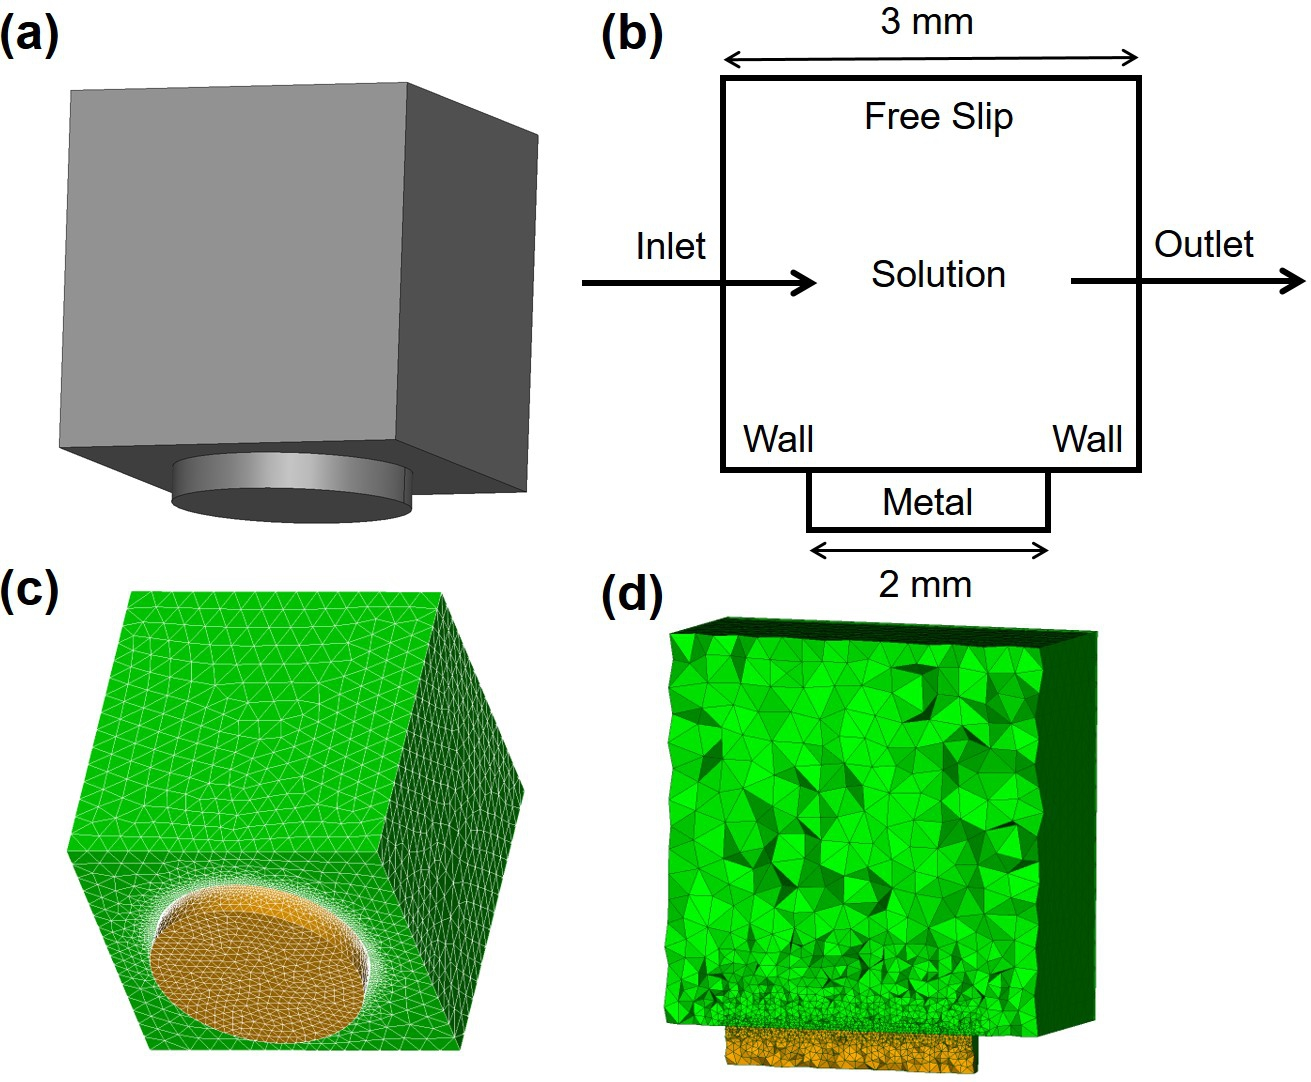
\includegraphics[width=\textwidth]{model_setup.jpg}
\caption[Computational model setup for local pH simulations]{Computational model setup for local pH simulations} \label{fig:kinetics_model_setup}
\end{figure}

The values of model parameters were set based on our previous work \cite{Barzegari2021}, but the following assumptions were also applied for selecting proper parameters of the coupled computational model:
\begin{enumerate}
\item
Diffusion rate of hydroxide ions is 5-10 times more than the rate of Mg ions, so $D_{\mathrm{OH}}$ was set as $D_{\mathrm{OH}} = 7.5 D_{\mathrm{Mg}}$ \cite{Gonzalez2021}.
\item
The hydroxyapatite-like precipitation doesn't forms immediately at the beginning and emerges later \cite{Gonzalez2021,Wang2022}. In the current model, it sets to start forming after the first hour of simulation time.
\item
The magnesium hydroxide layer is ticker at $37^{\circ}C$ \cite{Wang2022}, so the film elimination parameter ($k_2$) was set to be 50 times less in this temperature than the room temperate.
\end{enumerate}


%\section{Data Availability}
%
%The data used in the paper are available from the authors upon request.
%
%\section{Code Availability}
%The source code of the programs used in this paper is available from the authors upon request.
%
%
%\section{Acknowledgements}
%
%\section{Author Contributions}
%
%\section{Competing Interests}


%%%%%%%%%%%%%%%%%%%%%%%%%%%%%%%%%%%%%%%%%%%%%%%%%%
% Keep the following \cleardoublepage at the end of this file,
% otherwise \includeonly includes empty pages.
\cleardoublepage
